\documentclass{beamer}

\usepackage{amssymb}
\usepackage{amsfonts}
\usepackage{amsmath}
\usepackage{amsthm}
\usepackage{setspace}
\usepackage{longtable}
\usepackage{graphicx}
\usepackage{mathtools}
\usepackage{color}
\usepackage{array}
\usepackage{calc} 
\usepackage{bm}
\usepackage{caption}
\usepackage{float}


\usetheme{CambridgeUS}
\useoutertheme{infolines}
%numbering
\setbeamercolor{background canvas}{bg=white}
\setbeamersize{text margin left=1cm,text margin right=1cm}

\title[AI1110  Assignment-4]{ASSIGNMENT-4}
\subtitle{AI1110}
\author[]{MUKUNDA REDDY \\ AI21BTECH11021}
\date{}
\begin{document}
 
  \begin{frame}
      \titlepage
  \end{frame}
  
  \begin{frame}
      \tableofcontents
  \end{frame}
  
  \section{Question}
   \begin{frame}{Example 2-7}
   A telephone call occurs at random in the interval $(0, T)$.
   Find the probability that the call will occur in the interval
   $(t_1,t_2)$?
    \end{frame}
    
    \section{solution}
    \begin{frame}{Solution}
        Here S consists of noncountable infinity of elements so assigning individual probabilities is not possible.Lets consider the intervals and a function
        $\alpha(x)$\;which gives probability density such that\\
    \begin{equation}
    \label{normalization}
        \int_{-\infty}^{\infty} \alpha(x) dx = 1
    \end{equation}
    
    \end{frame}
    
    \begin{frame}{Solution}
    The probability of the event ${X_1 < X < X_2}$
    consisting of all points in the interval $(X_1, X_2)$
    is given by \\
    \begin{equation}
    \label{intervalprob}
        P(X_1<X<X_2) =  \int_{X_2}^{X_1} \alpha(x)dx 
    \end{equation}
    We can assign probability $\alpha(x) = 0$,for $-\infty<x<0$ and $T<x<\infty$ as there are no phone calls in that time period. \\
    \end{frame}
    
    \begin{frame}{Solution}
    Given call occurs randomly in interval $(0,T)$ meaning
    $\alpha(x)$ is uniform as it must satisfy the  let $\alpha(x) = c$ as this must satisfy \eqref{normalization},
    \begin{align*}
        \int_{-\infty}^{\infty} \alpha(x) dx &= \int_{-\infty}^{0} \alpha(x) dx  +\int_{0}^{T} \alpha(x) dx  +\int_{T}^{\infty} \alpha(x) dx \\
          &= 0+\int_{0}^{T} c dx +0 \: \text{(as $\alpha(x) =constant c$)} \\
          &= c(T) \\
    \end{align*}
    
    
    \end{frame}
    
     \begin{frame}{Solution}
     \begin{align}
         \implies \int_{-\infty}^{\infty} \alpha(x) dx &= 1 \\ \nonumber
          c(T) &= 1 \\ \nonumber
           c &= \frac{1}{T}
     \end{align}
     The probaility disttribution function is given by
         \[ 
    \alpha(x) = 
  \begin{cases}
    \frac{1}{T}, & if \; 0\le x \le T \\
    0, & \text{otherwise}
  \end{cases} 
         \]
     \end{frame}
     
     \begin{frame}{Solution}
         \begin{figure}
             \centering
             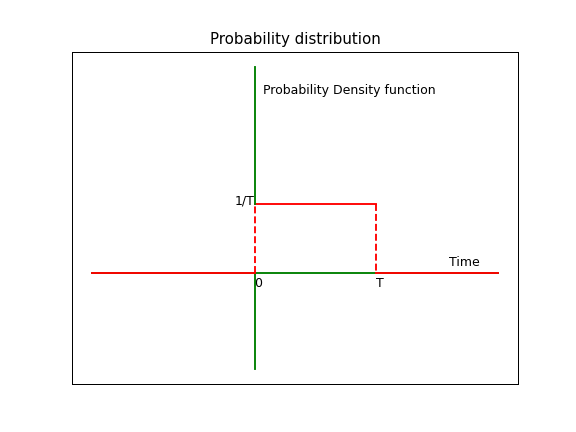
\includegraphics[scale=0.5]{Figure_1.png}
             \caption{y = \alpha(x)}
             \label{fig:my_distribution}
         \end{figure}
     \end{frame}
     
     \begin{frame}{Solution}
     From equation \eqref{intervalprob} we can write the
     probability of the  event {the call} will occur in the
     interval $(t_1,t_2)$ equals,
     \begin{align*}
         P(t_1 \le X \le t_2) &=  \int_{t_2}^{t_1} \alpha(x)dx \\
                      &=  \int_{t_2}^{t_1} \frac{1}{T}dx \\
                      &=   \frac{t_2-t_1}{T}.
     \end{align*}
     \end{frame}



\end{document}